\documentclass[14pt]{extarticle}
\usepackage[utf8]{inputenc}
\usepackage[T1]{fontenc}
\usepackage[spanish,es-lcroman]{babel}
\usepackage{amsmath}
\usepackage{amsthm}
\usepackage{physics}
\usepackage{tikz}
\usepackage{float}
\usepackage{calc}
\usepackage[autostyle,spanish=mexican]{csquotes}
\usepackage[per-mode=symbol]{siunitx}
\usepackage{gensymb}
\usepackage{multicol}
\usepackage{enumitem}
\usepackage{setspace}
\usepackage[left=2.00cm, right=2.00cm, top=2.00cm, 
     bottom=2.00cm]{geometry}
\usepackage{Estilos/ColoresLatex}
\usepackage{makecell}

% \usepackage[sfdefault]{roboto}  %% Option 'sfdefault' only if the base font of the document is to be sans serif
% \usepackage[T1]{fontenc}

\usepackage{scalerel}[2016-12-29]
\def\stretchint#1{\vcenter{\hbox{\stretchto[440]{\displaystyle\int}{#1}}}}
\def\scaleint#1{\vcenter{\hbox{\scaleto[3ex]{\displaystyle\int}{#1}}}}
\def\bs{\mkern-12mu}

\newcommand{\textocolor}[2]{\textbf{\textcolor{#1}{#2}}}
\sisetup{per-mode=symbol}
\decimalpoint
\sisetup{bracket-numbers = false}
\newlength{\depthofsumsign}
\setlength{\depthofsumsign}{\depthof{$\sum$}}
\newcommand{\nsum}[1][1.4]{% only for \displaystyle
    \mathop{%
        \raisebox
            {-#1\depthofsumsign+1\depthofsumsign}
            {\scalebox
                {#1}
                {$\displaystyle\sum$}%
            }
    }
}

\title{\vspace*{-2cm} Lentes delgadas}
\date{ }

\begin{document}
\maketitle

\section{Lentes delgadas.}

Una lente es una placa de vidrio cuyas caras son por lo general esféricas y casi paralelas en el centro de ella. Consideremos un haz de rayos paralelos que inciden en una lente muy delgada. Si la lente hace que los rayos refractados converjan, se dice que la lente es convergente, y si hace que diverjan, que la lente es divergente. También se dice que una lente divergente es negativa y que una convergente es positiva.

Si el medio que rodea a la lente es menos denso que el material con que está hecha la lente, una lente más elgada en su centro que en su periferia es divergente y una más gruesa en su centro que en su periferia es convergente. Las lentes delgadas pueden tener cualquiera de las formas que se muestran en la siguiente figura:
\begin{figure}[H]
    \centering
    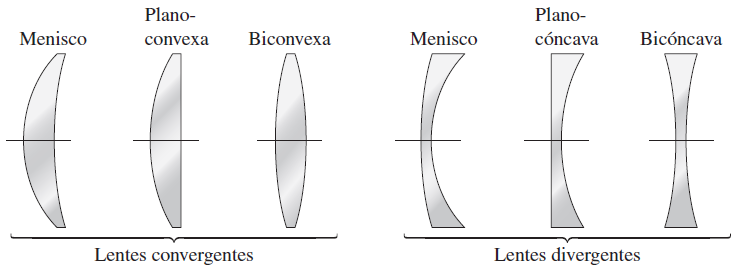
\includegraphics[scale=0.75]{Imagenes/Lentes_01.png}
    \caption{Tipos de lentes convergentes y divergentes.}
\end{figure}
Si la lente tiene dos superficies esféricas, el eje óptico es una línea imaginaria que pasa por los centros de la curvatura de ambas superficies. Si la lente tiene una superficie esférica y una plana, el eje óptico es una línea imaginaria perpendicular a la superficie plana que pasa por el centro de curvatura de la otra superficie. Es fácil ver con estas definiciones que el eje óptico pasa por la parte más gruesa o más delgada de la lente, según sea convergente o divergente, respectivamente.

El foco de una lente se define como el punto de convergencia de los rayos luminosos cuando éstos llegan a la lente en un haz de rayos paralelos entre sí y al eje de la lente. En una lente divergente el foco es el punto de convergencia de las prolongaciones de los rayos refractados. La distancia focal de una lente delgada es la distancia de la lente al foco, siendo positiva para una lente convergente y negativa para una lente divergente.
\begin{figure}[H]
    \centering
    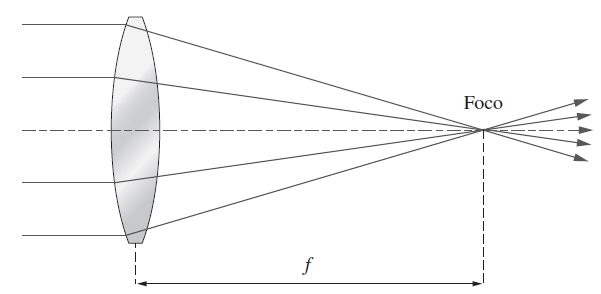
\includegraphics[scale=0.75]{Imagenes/Lentes_02.png}
    \caption{Lente convergente}
\end{figure}
\begin{figure}[H]
    \centering
    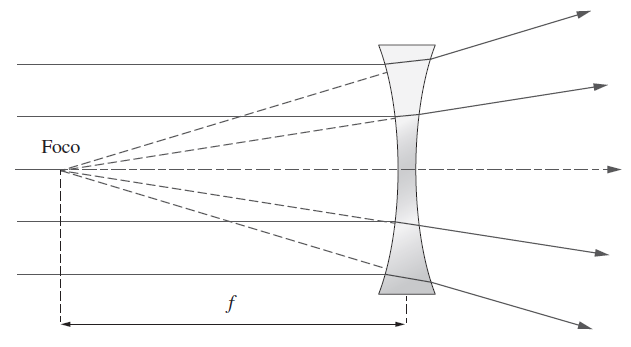
\includegraphics[scale=0.75]{Imagenes/Lentes_03.png}
    \caption{Lente divergente}
\end{figure}
La potencia $P$ de una lente se define como el recíproco de la distancia focal $f$:
\begin{align}
P = \dfrac{1}{f}
\label{eq:ecuacion_II_01}
\end{align}
si la distancia focal se mide en metros, la potencia queda expresada en dioptrías.

\subsection{Fórmula para lentes delgadas.}

Esta fórmula se puede encontrar aplicando la fórmula de Gauss a ambas caras de la lente. Así, para la primera superficie tenemos:
\begin{align}
\dfrac{n^{\prime}_{1}}{l^{\prime_{1}}} - \dfrac{n_{1}}{l_{1}} = \dfrac{n_{1}^{\prime} - n_{1}}{r_{1}}
\label{eq:ecuacion_II_02} 
\end{align}
donde las distancias $l_{1}$ y $l_{1}^{\prime}$ están ilustradas en la figura x.
\begin{figure}[H]
    \centering
    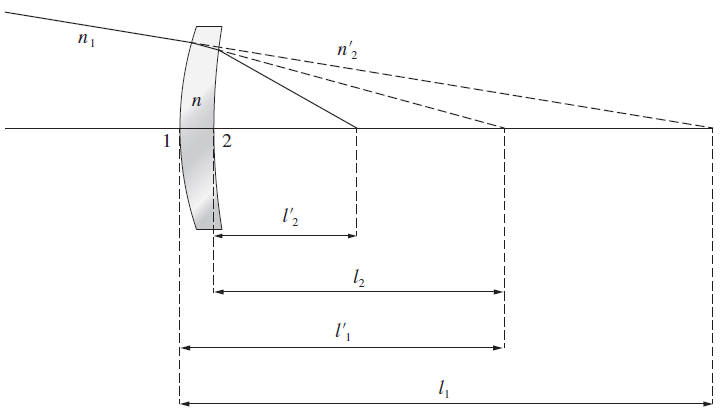
\includegraphics[scale=0.75]{Imagenes/Lentes_04.png}
    \caption{Refracción de un rayo luminoso meridional en una lente delgada.}
    \label{fig:figura_II_03}
\end{figure}
Haciendo lo mismo para la segunda superficie:
\begin{align}
\dfrac{n^{\prime}_{2}}{l^{\prime_{2}}} - \dfrac{n_{2}}{l_{2}} = \dfrac{n_{2}^{\prime} - n_{2}}{r_{2}}
\label{eq:ecuacion_II_03} 
\end{align}
El índice de refracción de la lente es $n$, por lo que podemos observar que:
\begin{align}
n_{1}^{\prime} = n_{2}^{\prime} = n
\label{eq:ecuacion_II_04}
\end{align}
Los índices $n_{1}$ y $n_{2}$ son en general igual a $1$, pero no siempre, ya que una de las caras de la lente puede estar en contacto con aceite o con agua. Si el grueso de la lente es muy pequeño comparado con la distancia, podemos escribir aproximadamente:
\begin{align}
l_{2} = l_{1}^{\prime}
\label{eq:ecuacion_II_05}
\end{align}
por lo que, sustituyendo las ecuaciones (\ref{eq:ecuacion_II_04}) y (\ref{eq:ecuacion_II_05}) en las ecuaciones (\ref{eq:ecuacion_II_02}) y (\ref{eq:ecuacion_II_03}) obtenemos:
\begin{align}
\dfrac{n}{l_{2}} - \dfrac{n_{1}}{l_{1}} = \dfrac{n - n_{1}}{r_{1}}
\label{eq:ecuacion_II_06}
\end{align}
y
\begin{align}
\dfrac{n_{2}^{\prime}}{l_{2}^{\prime}} - \dfrac{n}{l_{2}} = \dfrac{n_{2}^{\prime} - n}{r_{2}}
\label{eq:ecuacion_II_07}
\end{align}
sumando estas dos expresiones, miembro a miembro, resulta:
\begin{align}
\dfrac{n_{2}^{\prime}}{l_{2}^{\prime}} - \dfrac{n_{1}}{l_{1}} = \dfrac{n_{2}^{\prime} - n}{r_{2}} + \dfrac{n - n_{1}}{r_{1}}
\label{eq:ecuacion_II_08}
\end{align}
donde $l_{1}$ y $l_{2}^{\prime}$ son las distancias del objeto y de la imagen, respectivamente, a la lente. Estas distancias siguen la convención de signos introducidos en la sección anterior. 

Dada una lente delgada, el lado derecho de la ecuación (\ref{eq:ecuacion_II_08}) es una constante, por lo que el lado izquierdo de la misma ecuación debe ser la misma constante, aunque $l_{2}^{\prime}$ y $l_{1}$ sean individualmente variables. Supongamos el caso particular en que el objeto está a una distancia infinita y por lo tanto los rayos luminosos llegan a la lente en un haz de rayos paralelos entre sí y al eje óptico. En este caso $n_{1}/l_{1}$ es cero y $l_{2}^{\prime}$ es, por definición, igual a la distancia focal $f_{2}$. (Se usa el subíndice $2$ en $f$ para denotar que es la distancia de la lente al foco a la derecha de la lente; por lo tanto se usaría el subíndice $1$ para la otra distancia.) Podemos ver entonces que ambos lados de la ecuación (\ref{eq:ecuacion_II_08}) son iguales a $n_{2}^{\prime}/f_{2}$.

Igualando el lado derecho de la ecuación (\ref{eq:ecuacion_II_08}) a $n_{2}^{\prime}/f_{2}$ obtenemos:
\begin{align}
\dfrac{1}{f_{2}} = \dfrac{n - n_{1}}{n_{2}^{\prime} \, r_{1}} + \dfrac{n_{2}^{\prime} - n}{n_{2}^{\prime} \, r_{2}}
\label{eq:ecuacion_II_09}
\end{align}
Si el haz de rayos paralelos viaja de derecha a izquierda, el foco está a la izquierda de la lente. En este caso $n_{2}^{\prime}/l_{2}^{\prime}$ se hace cero y $l_{1}$ es, por definición, la distancia
focal $f_{1}$. Por lo tanto, de la misma ecuación (\ref{eq:ecuacion_II_08}) podemos obtener:
\begin{align}
\dfrac{1}{f_{1}} = \dfrac{n - n_{1}}{n_{1} \, r_{1}} + \dfrac{n_{2}^{\prime} - n}{n_{1} \, r_{2}}
\label{eq:ecuacion_II_10}
\end{align}
De las ecuaciones (\ref{eq:ecuacion_II_09}) y (\ref{eq:ecuacion_II_10}) podemos fácilmente concluir que las dos distancias focales $f_{2}$ y $f_{1}$ están relacionadas por:
\begin{align}
\dfrac{n_{2}^{\prime}}{f_{2}} = \dfrac{n_{1}}{f_{1}}
\label{eq:ecuacion_II_11}
\end{align}
Consideremos ahora el caso particular, muy común, en que la lente está rodeada de aire $(n_{2}^{\prime} = n_{1} = 1)$. En estas condiciones las dos distancias focales son idénticas $(f_{2} = f_{1} = f)$ y por consiguiente podemos escribir:
\begin{align}
\dfrac{1}{f} = (n -1) \left( \dfrac{1}{r_{1}} - \dfrac{1}{r_{2}} \right)
\label{eq:ecuacion_II_12}
\end{align}
Ésta es la llamada \textit{fórmula del fabricante de lentes}, válida únicamente para una lente delgada rodeada de aire y considerando rayos paraxiales.

Ésta es la llamada fórmula del fabricante de lentes, válida únicamente para una
lente delgada rodeada de aire y considerando rayos paraxiales.

\section{Formación de imágenes.}

La función primordial de una lente es formar imágenes, por lo que es deseable estudiar esta propiedad de las lentes con algún detalle.

\subsection{Puntos conjugados y amplificación lateral.}

De acuerdo con lo visto en la sección anterior es posible igualar ahora el lado izquierdo de la ecuación \ref{eq:ecuacion_II_08} a $n_{2}^{\prime}/f_{2}$, con lo que obtenemos:
\begin{align}
\dfrac{1}{f_{2}} = \dfrac{1}{l_{2}^{\prime}} - \dfrac{n_{1}}{n_{2}^{\prime} \, l_{1}}
\label{eq:ecuacion_II_13}
\end{align}
Pero si $n_{1} = n_{2}^{\prime}$, esta expresión se reduce a:
\begin{align}
\dfrac{1}{f} = \dfrac{1}{l_{2}^{\prime}} - \dfrac{1}{l_{1}}
\label{eq:ecuacion_II_14}
\end{align}
Con esta relación podemos calcular la posición de la imagen, dada la posición del objeto y la distancia focal. Las posiciones del objeto y su imagen superficierespectiva sobre el eje óptico se dice que son dos \textit{puntos conjugados}.

La ecuación (\ref{eq:ecuacion_II_13}) también se puede obtener usando la ecuación (\ref{eq:ecuacion_II_11}) y la definición de distancia focal. Por la definición de distancia focal, un rayo que llega a la lente paralelo al eje óptico pasa por el foco $F_{2}$. En forma simultánea un rayo que llega a la lente después de pasar por el foco $F_{1}$ saldrá de ella paralelo al eje óptico.
Como se muestra en la figura (\ref{fig:figura_II_04}) el rayo $1$ llega paralelo al eje óptico y por lo tanto pasa por el foco $F_{2}$ después de refractarse. El rayo $2$ pasa por $F_{1}$, por lo que sale de la lente paralelo al eje óptico.
\begin{figure}[H]
    \centering
    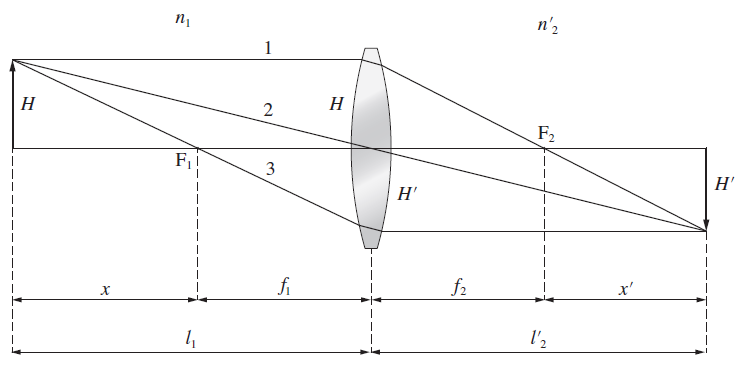
\includegraphics[scale=0.75]{Imagenes/Lentes_05.png}
    \caption{Posiciones del objeto y la imagen, o puntos conjugados.}
    \label{fig:figura_II_04}
\end{figure}
En la figura (\ref{fig:figura_II_04}) las distancias $l_{1}$ y $H^{\prime}$ son negativas, de acuerdo con nuestra notación de signos ya establecida. Las distancias $x$ y $x^{\prime}$ de la figura x quedan dadas por:
\begin{eqnarray}
x^{\prime} &= l_{2}^{\prime} - f_{2} \label{eq:ecuacion_II_15} \\[0.5em]
x &= - l_{1} - f_{1} \label{eq:ecuacion_II_16}
\end{eqnarray}
Considerando el lado izquierdo de la lente tenemos que:
\begin{align}
\dfrac{H}{-H} = \dfrac{x}{f_{1}}
\label{eq:ecuacion_II_17}
\end{align}
y considerando el lado derecho:
\begin{align}
\dfrac{H}{-H^{\prime}} = \dfrac{f_{2}}{x^{\prime}}
\label{eq:ecuacion_II_18}
\end{align}
de donde, igualando estas dos expresiones, se obtiene:
\begin{align}
x \, x^{\prime} = f_{1} \, f_{2}
\label{eq:ecuacion_II_19}
\end{align}
Ésta es la forma en la que Newton relacionó las posiciones del objeto y su imagen, por lo que a esta expresión se la conoce como fórmula de Newton.

Si sustituimos en la fórmula de Newton los valores de $x$ y $x^{\prime}$ dados por las ecuaciones
(\ref{eq:ecuacion_II_15}) y (\ref{eq:ecuacion_II_16}) obtenemos:
\begin{align}
\dfrac{1}{f_{2}} = \dfrac{1}{l_{2}^{\prime}} - \dfrac{f_{1}}{f_{2} \, l_{1}}
\label{eq:ecuacion_II_20}
\end{align}
y, finalmente, combinando la ecuación (\ref{eq:ecuacion_II_20}) con la ecuación (\ref{eq:ecuacion_II_11}) obtenemos la ecuación (\ref{eq:ecuacion_II_13}) como esperábamos.

Al igual que en el tema anterior, la amplificación lateral de una lente está definida como:
\begin{align}
m = \dfrac{H^{\prime}}{H}
\label{eq:ecuacion_II_21}
\end{align}
Por lo tanto, de las ecuaciones (\ref{eq:ecuacion_II_18}) y (\ref{eq:ecuacion_II_15}) se puede ver que:
\begin{align}
m = - \dfrac{x^{\prime}}{f_{2}} = 1 - \dfrac{l_{2}^{\prime}}{f_{2}}
\label{eq:ecuacion_II_22}
\end{align}
Usando ahora el valor de $f_{2}$ de la ecuación (\ref{eq:ecuacion_II_13}) obtenemos la siguiente expresión para la amplificación lateral:
\begin{align}
m = \dfrac{n_{1} \, l_{2}^{\prime}}{n_{2}^{\prime} \, l_{1}}
\label{eq:ecuacion_II_23}
\end{align}
cuando $n_{1} = n_{2}^{\prime}$, esta relación se reduce a:
\begin{align}
m = \dfrac{l_{2}^{\prime}}{l_{1}}
\label{eq:ecuacion_II_24}
\end{align}
Si igualamos la ecuación (\ref{eq:ecuacion_II_24}) con la (\ref{eq:ecuacion_II_21}) podemos demostrar que un rayo que pase por el centro de una lente delgada no cambia su dirección después de salir de la lente si y solamente si $n_{1} = n_{2}^{\prime}$.

\subsection{Lentes convergentes.}

La formación de imágenes por medio de lentes convergentes se puede estudiar más fácilmente graficando en un diagrama las posiciones $l_{2}^{\prime}$ de la imagen contra las posiciones $l_{1}$ del objeto, como se muestra en la figura (\ref{fig:figura_II_05}).
\begin{figure}[H]
    \centering
    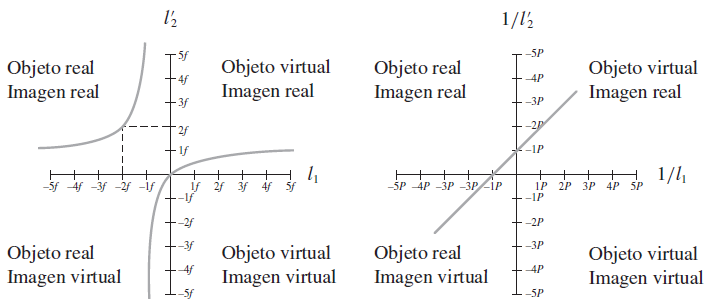
\includegraphics[scale=0.75]{Imagenes/Lentes_06.png}
    \caption{Posiciones del objeto y la imagen con lentes convergentes. $P$ es la potencia 1/distancia.}
    \label{fig:figura_II_05}
\end{figure}
Como se puede observar en esta figura, no es posible con una lente convergente obtener imágenes virtuales con objetos virtuales. Además, podemos ver que la imagen pasa bruscamente de real a virtual cuando el objeto pasa por el foco de la lente al irse acercando a ella. Las tres combinaciones posibles de tipos de objeto e imagen que se puede formar con una lente convergente se ilustran de manera clara en las figuras (\ref{fig:figura_II_06a}) a (\ref{fig:figura_II_06c}).
\begin{figure}[H]
    \centering
    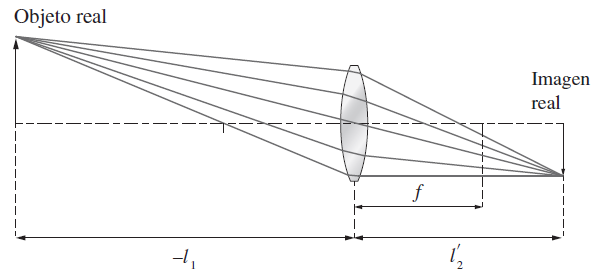
\includegraphics[scale=0.8]{Imagenes/Lentes_07a.png}
    \caption{Tipos de imágenes
formadas con lentes convergentes.}
    \label{fig:figura_II_06a}
\end{figure}
\begin{figure}[H]
    \centering
    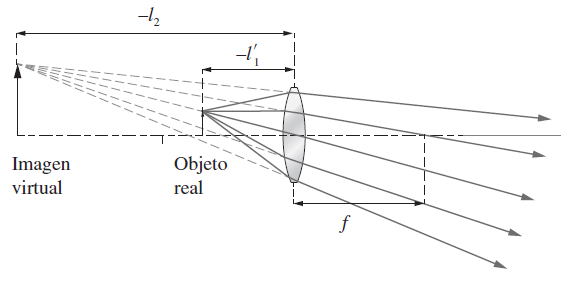
\includegraphics[scale=0.8]{Imagenes/Lentes_07b.png}
    \caption{Tipos de imágenes formadas con lentes convergentes.}
    \label{fig:figura_II_06b}
\end{figure}
\begin{figure}[H]
    \centering
    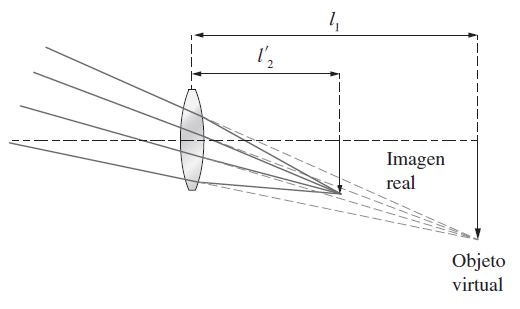
\includegraphics[scale=0.8]{Imagenes/Lentes_07c.png}
    \caption{Tipos de imágenes
formadas con lentes convergentes.}
    \label{fig:figura_II_06c}
\end{figure}
En el siguiente cuadro se tabulan algunos parámetros para los tres casos de combinaciones de objeto e imagen con lentes convergentes.
\begin{table}[H]
    \centering
    \begin{tabular}{l c c c}
        Limites en la pos. objeto & $-\infty, F_{1}$ (real) & $F_{1}$, lente (real) & Lente, $+\infty$ (virtual) \\ \hline
        Tipo de imagen & Real & Virtual & Real \\
        Signo de $l_{2}^{\prime}$ & $+$ & $-$ & $+$ \\
        Signo de $m$ & $-$ & $+$ & $+$ \\
        Magnitud de $m$ & $>< 1$ & $> 1$ & $< 1$        
    \end{tabular}
\end{table}
\end{document}